
% Paper to be submitted to Ocean and Atmospheric Data Management
% (http://oxford.elsevier.com/cgi-bin/JAO/C-/pass?OADM). 2/4/99 jhrg
%
% $Id$

\documentclass[12pt]{article} 
\usepackage{epsfig,alltt,harvard,acronym}
\bibliographystyle{agsm}
\newcommand{\Cpp}{{\rm {\small C}\raise.5ex\hbox{\footnotesize ++}}}

\begin{document}

\title{Experience Building The Distributed Oceanographic Data System}

\author{James Gallagher\footnote{The University of Rhode Island, South Ferry
    Rd., Narragansett, RI. 02882 email: jgallagher@gso.uri.edu,
    pcornillon@gso.uri.edu, tomss@ids.com} 
  \and Peter Cornillon\footnotemark[1]
  \and Tom Sgouros\footnotemark[1]
  \and Glenn Flierl\footnote{The Massachusetts Institute of Technology,
    Cambridge, MA. email: glenn@lake.mit.edu}}

\date{\today}

\maketitle
% PCC 2/18/99 changed all 'data set*' to 'dataset*'

\begin{abstract}
  
  In this paper we present an overview of the \ac{DODS} and discuss the
  impact of some of the more important design considerations on system
  performance. \ac{DODS} addresses standardization on two fronts: uniform
  transport of data stored in many formats and access to that transport by
  many programs, including legacy software. \ac{DODS} uses \acs{HTTP} to
  implement a transaction-based client-server system and has a simple data
% PCC 2/18/99 removed 'a' before general
%  model which closely mirrors that of a general purpose programming languages
  model which closely mirrors that of general purpose programming languages
  with a few extensions for science data. Metadata are processed separately
  from the data type and value information by the system and the inclusion of
  metadata has been structured so that data providers may, via an ancillary
  file, add to a dataset's metadata at any time without modifying the
  dataset.  Furthermore, datasets may be added to the system regardless of
  how much metadata they have. Legacy software can access \ac{DODS} servers
  transparently using recoded implementations of existing data access
  \acs{API}s, and clients that access \ac{DODS} servers can do so under
  program control; they are not limited to stand-alone operation. We have
  found that this transaction-based client-server system with its simple data
% TS 2/18/99 fare ==> faire
%  model and laissez-fare attitude toward metadata provides for a flexible
  model and laissez-faire attitude toward metadata provides for a flexible
  balance between broad and deep interoperability that allows the
% TS 2/18/99 fare ==> faire
%  provider/user communities to tailor system components for their needs.
  data provider and user communities to tailor system components for their
  needs. 
 
\end{abstract}

{\bf Keywords:} Oceanographic data, distributed data systems, remote access.

\tableofcontents

\section{Introduction}

% This portion of the paper originally appeared in RV Tech. The CVS ID for
% that doc was:  
%       `rvtec.tex,v 1.1 1995/07/12 19:45:22 george Exp'
%
% I've also used it as the introduction to a 1995 paper that appeared in the
% WWW Journal (O'Reilly & Asoc.). Is this getting over used? 2/5/99 jhrg
% I've since modified the text a fair bit. 2/12/99 jhrg

% PCC 2/18/99 added footnote
% It does not take long using the \ac{WWW} to discover many hundreds of
It does not take long using the \ac{WWW}\footnote{All acronyms are
defined in Appendix A. Some of the more common acronyms such as URL
are not expanded in the text.} to discover many hundreds of
scientific datasets that are currently available on-line to researchers.  For
oceanographers the volume and diversity of data from national archives,
special program offices or other researchers that is of potential value to
their research is overwhelming. However, while a large number of
oceanographic datasets are on-line, from the research oceanographer's point
of view there are significant impediments which often make acquiring and
using these on-line data hard \cite{muntz:data}.

Many data archive centers have developed their own data management systems
with specialized interfaces for navigating their data resources. Examples of
such systems include the \acs{NASA}-\acs{JPL} \acs{AVHRR} Oceans Pathfinder
% PCC 2/18/99 my version can not find citation to podaac:sst
Homepage \cite{podaac:sst}, the \acs{EOSDIS} \acs{IMS} data ordering system
\cite{eosdis:ims} and the \acs{NOAA}-\acs{PMEL} Web Access to Oceanographic
% PCC 2/18/99 my version can not find citation to noaapmel:tao
in-situ Data \cite{noaapmel:tao}.  Virtually none of these data systems
% PCC 2/18/99 interoperate is cumbersome.
% interoperate with each other beyond using a web browser as an interface
are accessible from the others beyond using a web browser as an interface
display tool, making it necessary for a user to visit many systems and learn
multiple interfaces in order to acquire data.

In parallel with the development of web interfaces to data holdings, there
has been increased activity in the deployment of standard storage policies
for various types of data within the oceanographic community. For example,
The University Corporation for Atmospheric Research, though its Unidata
program, has established a repository of standard conventions which have been
% TS 2/18/99 Atmospheric spelled wrong in citation ==> netcde:conventions
developed by the \acs{NetCDF} user community \cite{netcdf:conventions}.
Similarly, there is a strong ongoing effort to establish metadata standards
within the \acs{HDF} user community \cite{hdfeos}. However, these standards
only address transfer of information within the scope of a particular file
format.
% PCC 2/16/99 You might also mention that these data formats do not work
% across the net!
% 2/16/99 jhrg: I don't think that's true. You could use NFS to access the
% files over the net work.
% TS 2/18/99 acronym has 'i' in 'interface' in lower case.
Because these formats have an associated \ac{API}, it is possible for
knowledgeable programs to tap into this standard, but only within the scope
% TS 2/18/99 change
% of a particular \ac{API}. Thus, it is difficult to view or combine several
of the corresponding \ac{API}. Thus, it is difficult to view or combine several
datasets if they use different storage formats even though, as
\citeasnoun{pursch:newtools} point out, combining datasets is often a key
requirement of global-scale earth science.  This is particularly troublesome
because it is often the case that the information underlying these datasets
is fundamentally compatible.

Finally, while large data centers have a clearly defined data policy, and
often a mandate, to make data accessible to members of the research community
\cite{noaa:policy}, there is scant infrastructure that enables individual
scientists to make data accessible to others in a simple way. While many
scientists in the earth-sciences community share data, and cite shared data
as one of their most important resources, doing so is often cumbersome
\cite{dods:workshop1}. Systems like the World Wide Web make sharing research
results vastly simpler, but do little to reduce the difficulty of sharing raw
data.

% PCC 2/18/99 added acronyms.
% To address these problems, researchers at the University of Rhode Island and
% the Massachusetts Institute of Technology are creating a network tool that,
To address these problems, researchers at the University of Rhode Island 
(URI) and the Massachusetts Institute of Technology (MIT) are creating a 
network tool that,
while taking advantage of \ac{WWW} data resources, helps to resolve the issue
of multiple data formats and different data systems interfaces.  This network
tool, called the \acf{DODS}, enables oceanographers to interactively access
% TS 2/18/99 'the one' ==> 'an'
% distributed, on-line science data using the one interface that a researcher
distributed, on-line science data using an interface that a researcher
is already familiar with --- existing data analysis application software (i.e.,
legacy systems) --- while at the same time providing a set of tools which can be
used to build new application software specifically intended to work with
distributed resources.  The architecture and design of \ac{DODS} makes it
possible for a researcher to open, read, subsample and import directly into
his or her data analysis applications scientific data resources using the
\ac{WWW}.  The researcher does not need to know either what format is used to
store the data or how the data is actually accessed and served by the remote
data system \cite{gallagher:dods}.

In the remainder of this paper we present an overview of \ac{DODS} and
discussion of the system's strengths and weaknesses. In
section~\ref{overview} we present the general architecture of \ac{DODS}
including a description of client-server design (section~\ref{cs}), the data
model and metadata model (sections~\ref{dm} and~\ref{md}), the use of
\acs{URL}s by the system (section~\ref{url}) and a brief description of the
implementation of servers (section~\ref{servers}) and clients
(section~\ref{clients}). In the second part of the paper, discussion
(section~\ref{disc}), we examine the tradeoffs of using \acs{HTTP}
(section~\ref{http}), the simple data model and metadata policy
(section~\ref{ddm} and~\ref{dmd}), the modular server design
(section~\ref{dserver}) and client designs (section~\ref{dclients}). In
section~\ref{conclusion} we present concluding remarks.

\section{Overview of \ac{DODS}}
\label{overview}

The architecture of \ac{DODS} grew from a few basic assumptions about the way
scientists use data \cite{dods:workshop1}. First, because scientists rank
data obtained from colleagues as very important, \ac{DODS} supports
scientists as data providers on a par with data centers. Second, while data
centers typically require that extensive documentation accompany a dataset
before it can be made generally available, an individual scientist might want
to make a dataset available without providing much information because his or
her colleagues may know enough about those data to use them ``as is.''  This
mirrors the common practice of tape or ftp exchange between scientists.

Though, as in such cases, extensive dataset documentation is not necessary, a
data system like \ac{DODS} \emph{can} provide a lot of information to a user.
Therefore, \ac{DODS} was designed to support various levels of metadata
starting at a low point where only the data types are known and ranging up to
very complete collections like those defined by \acs{NetCDF} \acs{COARDS}
\cite{netcdf:conventions} or \acs{HDF}-\acs{EOS} \cite{hdfeos}.

\subsection{\ac{DODS} is a client-server system}
\label{cs}

\ac{DODS} uses client-server architecture to provide access to data across
the Internet. By installing one or more \ac{DODS} data servers---standard
\acs{HTTP} servers, equipped with a set of \ac{DODS} \acs{CGI} programs---any
computer with on-line data can provide access to any user with network
access.  Users employ client programs to access data from the data servers by
connecting to them in a manner identical to the way a web browser retrieves a
web page.

The data delivery infrastructure for the entire system is the set of
\ac{DODS} data servers and clients in existence at any given time. Some servers will
be permanent; others will appear for special purposes and then be
taken off-line.  This is also
comparable to the situation of the World Wide Web.  In the near future there
will be a system which enables users to search for \ac{DODS} servers with a
particular type or location of data, but participation in such a central
registry will always be a voluntary part of the system.

The data delivery architecture does not rely on a centralized archive of
data; instead various data providers make relatively small amounts of data
available using their computers and data server software. Each user of data
% PCC 2/18/99 Comes across as DODS accessing the entire set of holding at once.
% can access the sum total of data from all sites making data available much as
can access any data from any site making data available much as
each user of a World Wide Web browser can access any document made available
through \acs{HTTP} servers. While the contribution from most sites is small,
the total pool of data that users can access is potentially very large; as of
% TS 2/18/99 modified
% 1 February 1999, in excess of 200GB of data were available from more than 10
1 February 1999, in excess of 200GB of data were available from over 10 different
sites.

\subsection{The DODS Data Model}
\label{dm}

% PCC 2/18/99 I am not sure about this one changed closely based.
% \ac{DODS} provides access to data using a simple data model closely based on
\ac{DODS} provides access to data using a simple data model based closely on
the file formats used in \acs{NetCDF} and \acs{HDF}. Within \ac{DODS},
datasets are composed of variables which have data types similar to those
found in programming languages such as C, with a few additions. In addition
to the common data types such as Byte, Integer, Float, String, Array and
Structure, \ac{DODS} also supports \acs{URL}s, Lists, Sequences and Grids.
The last two are of particular importance.

Sequences are used to store relational data such as would be found in a
relational database. Grids are used to store arrays that have mapping vectors
associated with their indices. The \ac{DODS} User's Guide
\cite{dods:users-guide} contains a more thorough explanation of these
data-types.  The addition of these two types makes it possible to represent
all the information that can be stored in either \acs{NetCDF} or \acs{HDF}.
In addition, we have built servers for several other file formats and several
relational database systems without difficulty.

\subsubsection{Metadata}
\label{md}

In addition to typed variables, \ac{DODS} supports the notion of \emph{data
  attributes}.  Bound to each variable in a dataset are one or more
type-name-value tuples called ``attributes.''  Each variable has, in effect,
a collection of attributes.  Each dataset may also have an arbitrary number
of other named collections of attributes not bound to any particular
variable. These two groups of attribute containers provide a way to encode
metadata that is compatible with the data formats and \ac{API}s \ac{DODS}
supports and is rich enough to support adding extra information.  The
attribute containers can also be named and nested, allowing \ac{DODS} to
support several metadata standards within the same dataset.

When a \ac{DODS} server is asked to return attribute information for a
dataset, it reads information from the dataset and then adds to it
information stored in an optional ancillary attribute file (see
Figure~\ref{fig:server-arch}). The ancillary attribute file is a simple yet
% PCC 2/18/99 Removed 'the' before 'metadata'; metadata is plural.
% powerful way to augment the metadata associated with a dataset without
powerful way to augment metadata associated with a dataset without
altering the dataset itself. This is an important
% PCC 2/16/99 This is confusing. In the previous sentence you are
% talking about metadata and in this sentence about data. I have
% not reworked it. The subsequent sentence continues the confusion.
% 2/16/99 jhrg Added some clarifying text. 
requirement of \ac{DODS}; that datasets can be added to \ac{DODS} without
% TS 2/18/99 'including' ==> 'such as'
% much effort on the part of the provider, including matching their dataset to
much effort on the part of the provider, such as matching their dataset to
% PCC 2/18/99 Last 2 sentences are confusing. I don't think they are needed.
% a complex metadata standard. However, to make datasets useful to a wide
% audience, metadata is often required. Because the optional ancillary metadata
% file is separate from the data itself, it is simple to add more metadata to a
% dataset once the \ac{DODS} server is set up.
a complex metadata standard. 

% PCC 2/18/99 Put figure 1 here after first reference to it.
\begin{figure}[htbp]
\begin{center}
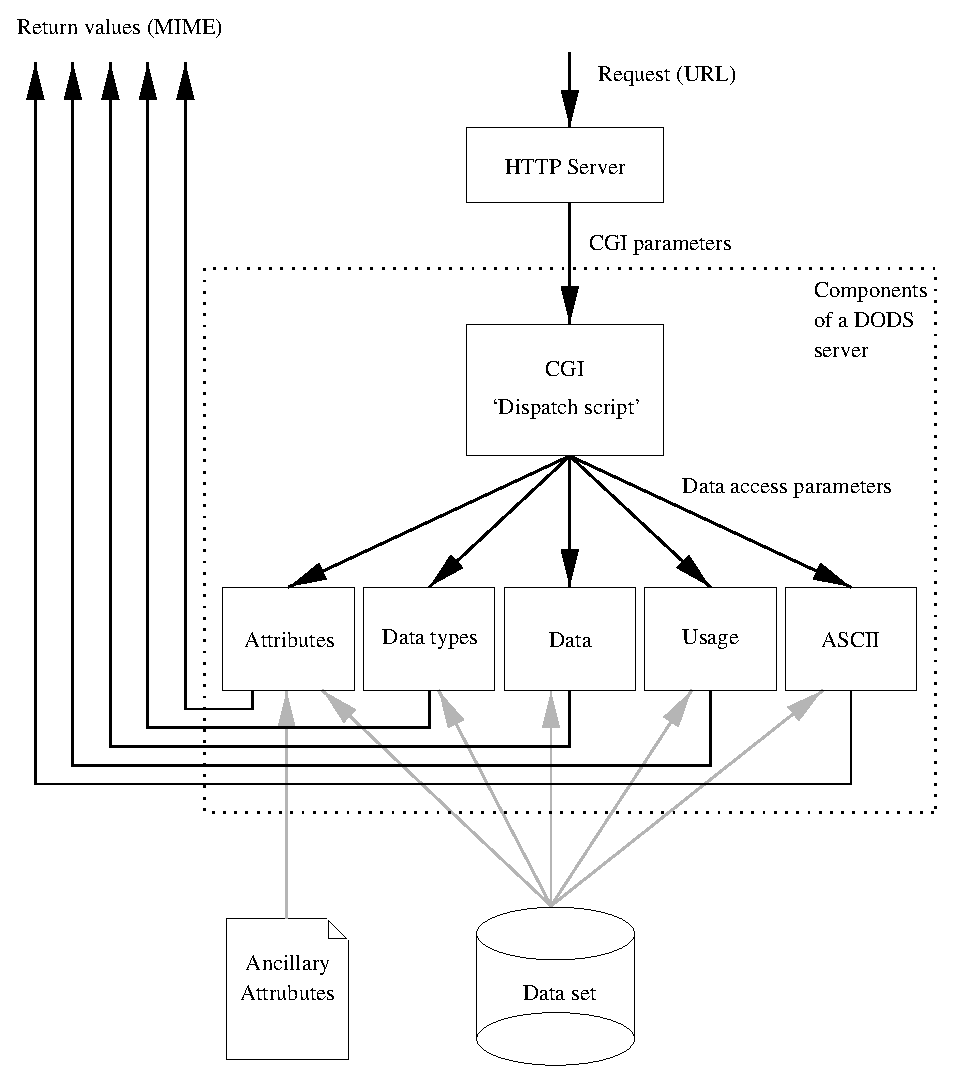
\epsfig{file=OADM-figs/server-arch.eps,width=5in}
\caption{A DODS server is composed of a CGI script and five UNIX
  filter  programs. The programs are run to produce the five different types of
  return information uses can request.}
\label{fig:server-arch}
\end{center}
\end{figure}

\subsection{URLs are used to refer to data}
\label{url}

Users or clients request data with \acs{URL}s. A \acs{URL} that requests data
% PCC 2/18/99 Removed DODS URL, you never use it.
% from a \ac{DODS} server (or `\ac{DODS} \acs{URL}') can be broken into four
from a \ac{DODS} server can be broken into four
parts: {\tt host}, {\tt CGI}, {\tt file}, and {\tt query}. The {\tt host}
part contains the Internet address of a machine running a \ac{DODS} server.
The {\tt CGI} component names the CGI dispatch script on that host which
serves as the user's interface with the \ac{DODS} server. The {\tt file} part
names a specific data file or other piece of information which is to be
% TS 2/18/99 Make footnote
% passed on to other parts of the server in order to complete the request. Note
% that the {\tt file} component does not have to actually be a file; for
% example the \ac{DODS}-JGOFS servers use this part of the \acs{URL} to name a
% dataset, and then uses that name when accessing the JGOFS data system.
passed on to other parts of the server in order to complete the 
request\footnote{Note
that the {\tt file} component does not have to actually be a file; for
example the \ac{DODS}-JGOFS servers use this part of the \acs{URL} to name a
dataset, and then uses that name when accessing the JGOFS data system.}.
Finally, any additional information needed for data access is passed in the
{\tt query} part of the \acs{URL}.

\begin{alltt}
    http://\emph{<host>}/cgi-bin/\emph{<CGI>}/\emph{<file>}?\emph{<query>}
\end{alltt}

The information passed to the \ac{DODS} server in the {\tt query} part of the
\acs{URL} bears special attention. The {\tt query} component is referred to
in the \ac{DODS} User's Guide \cite{dods:users-guide} as a constraint
% PCC 2/18/99 Removed 'the' before projection.
% expression. These expressions are divided into two parts: the projection and
expression. These expressions are divided into two parts: projection and
selection. The projection part is used to choose which variables from the
dataset will be returned, while the selection part is used to select from
% TS 2/18/99 modified
% among those variables' values those which meet certain criteria.
among those variables' the ones which  meet certain criteria.

The projection part can be used to subsample arrays or choose certain
variables from Structure, Sequence or Grid variables. The selection part can
be used to request that only those Sequence instances which satisfy a
relational expression be returned. The expressions are very powerful in that
they allow considerable flexibility in applying constraints to datasets. For
example, it is possible to write constraints not only in terms of constants
but also in terms of other variables in the dataset as well as other
variables in other \ac{DODS} datasets.

\begin{table}
% PCC 2/18/99 Sorry for changing my mind. Made the description a footnote
% \caption{Abbreviated Constraint Expression Production Rules.
% The table shows that
% \emph{expression} is composed of two parts, a \emph{projection} and a
% \emph{selection} part. In this table, literal items appear in bold face and
% alternatives are shown as multiple rules listed to the right. Thus
% a \emph{projection} can be either a single \emph{proj-term} or a list of
% \emph{proj-term}s separated by comma (,) characters. Note also that
% \emph{proj-term}s may also be null (indicated by the $\delta$).}
% \caption{Abbreviated Constraint Expression Production Rules}
% PCC 2/18/99 also added an extra blank line before the table.
\bigskip
\label{api:tab:expr}
\begin{center}
\begin{tabular}{lll} \hline

\emph{expression} & $\Rightarrow$ & \emph{projection} \emph{selection} \\

\emph{projection} & $\Rightarrow$ & \emph{proj-term} \\
                  &             & \emph{proj-term} {\tt ,} \emph{projection} \\
                  &             & $\delta$ \\

\emph{proj-term}  & $\Rightarrow$ & \emph{variable} \\
                  &             & \emph{function-returning-void}\\

\emph{selection}  & $\Rightarrow$ & {\tt \&} \emph{sel-term} \\
                  &             & {\tt \&} \emph{sel-term} \emph{selection} \\
                  &             & $\delta$ \\

\emph{sel-term}   & $\Rightarrow$ & \emph{rvalue} \emph{operator} \emph{rvalue} \\
                  &             & \emph{rvalue} \emph{operator} {\tt \{} 
                                         \emph{list of rvalues} {\tt \}} \\
                  &             & \emph{function-returning-boolean} \\

\emph{rvalue}     & $\Rightarrow$ & \emph{variable} \\
                  &             & \emph{literal} \\

\emph{operator}   & $\Rightarrow$ & ${\tt =} | {\tt !=} | {\tt <} | {\tt <=}
                                     | {\tt >} | {\tt >=}$ \\
\end{tabular}
\end{center}
\end{table}

Table~\ref{api:tab:expr} shows the complete constraint expression syntax
% PCC 2/18/99 Sorry for changing my mind. Made the description a footnote
%             and changed a few lines.
% using an abbreviated notation. Note that both the selection and projection
using an abbreviated notation\footnote{The table shows that
\emph{expression} is composed of two parts, a \emph{projection} and a
\emph{selection} part. Literal items appear in bold face and
alternatives are shown as multiple rules listed to the right. Thus
a \emph{projection} can be either a single \emph{proj-term} or a list of
\emph{proj-term}s separated by comma (,) characters. 
\emph{proj-term}s may also be null (indicated by the $\delta$).}. 
Note that both the selection and projection
parts of the expression can contain function calls. Functions called in the
projection part of the expression generally add new variables to the dataset
(and hence return no value) while functions called in the selection part
return boolean values. Every \ac{DODS} server supports a base set of
functions.  Each server can customize this by adding its own functions. These
function effectively add new operators for the data types. For example, while
a Grid is essentially an Array bound to map vectors and Arrays are not
\emph{selectable}, there is an implicit relation between the values of those
vectors at various indices and the values of the Array at those indices. That
relation suggests the possibility of selection. The \ac{DODS} servers have a
function which provide a way for clients to select a part of the Grid based
% TS 2/18/99 l.c.
% on the values of the Map vectors.  Thus, if the client knows that two map
on the values of the map vectors.  Thus, if the client knows that two map
vectors correspond to latitude and longitude, it is possible to use this
function to request those parts of the Grid that fall within certain ranges
of latitude and longitude.

% TS 2/18/99 Tom suggests not using math mode in the text. It's your call.
Note that the selection clauses are always combined using a boolean \emph{AND}
operation; there is no provision for \emph{OR}ing selection terms together.
However, as shown in the second production of the \emph{sel-term} rule,
operators can be used to compare an \emph{rvalue} to a list of
\emph{rvalues}. In this case the comparison returns true if \emph{operator}
is true for any one of the list elements, effectively providing the client
with the ability to perform boolean $OR$ operations within terms.

\subsection{The DODS Server}
\label{servers}

The \ac{DODS} server architecture is modular, as shown in
Figure~\ref{fig:server-arch}.  A \ac{DODS} server is built from
five\footnote{Five is a minimum figure.  A particular server installation may
  choose to install others.} separate UNIX filter programs (Attributes, Data
types, \ldots, in the figure) and a \ac{CGI} script.  The script is run by the
% PCC 2/18/99 this ==> the
% web server in response to a request for data. The web server passes this
web server in response to a request for data. The web server passes the
script values that were sent in the \acs{URL}. These values tell the dispatch
script which object the user wants and provide any special information (such
as sub-setting requests) that might be needed by the filter. The filter
programs interpret the parameters, read information from the dataset and
return an object encoded in a \acs{MIME} document.

% PCC 2/18/99 Moved figure 1 from here.
%\begin{figure}[htbp]
%\begin{center}
%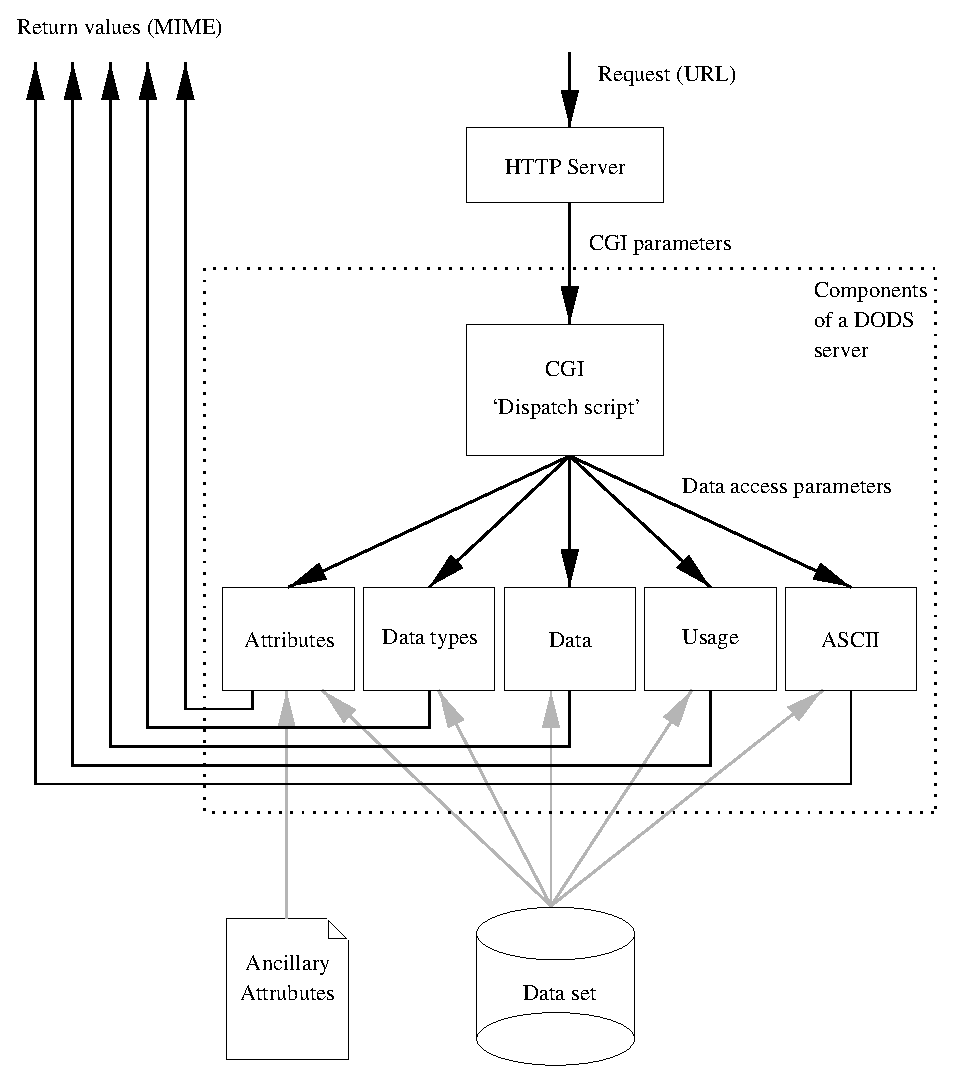
\epsfig{file=OADM-figs/server-arch.eps,width=5in}
%\caption{A \ac{DODS} server is composed of a \ac{CGI} script and five UNIX
%  filter  programs. The programs are run to produce the five different types of
%  return information uses can request.}
%\label{fig:server-arch}
%\end{center}
%\end{figure}

Building the filter programs is made easier by using a \Cpp\ library developed
as part of the project. This simplifies instantiating the objects which
comprise \ac{DODS} and creating network representations of those objects. The
\ac{DODS} \Cpp\ class library contains abstract classes for each of the data
types which \ac{DODS} supports. A server writer subclasses these creating
specializations for a particular data format or \ac{API}. Most servers follow
a set pattern with only minor variation.

\subsection{The DODS Client}
\label{clients}

% PCC 2/18/99 client ==> clients
% There are two classes of \ac{DODS} client, distinguished by the manner in
There are two classes of \ac{DODS} clients, distinguished by the manner in
which they use the tools provided in the \ac{DODS} software library.

\subsubsection{Legacy Clients}
\label{legacy}

The first class of \ac{DODS} clients were not designed with access to network
datasets in mind.  These are application programs built to analyze local
datasets on a user's own computer.  To use these programs, a researcher
originally would have had to find the data, import them to his or her own
computer, and then convert them to the file format required by the program,
such as \acs{NetCDF}.

For a limited number of \ac{API}s, such as \acs{NetCDF}, \ac{DODS} provides
drop-in replacement libraries with which a researcher can convert an existing
data analysis application into a specialized World Wide Web browser, capable
of requesting data from \ac{DODS} servers.  The conversion is accomplished
simply by relinking the program with the \ac{DODS} version of the \ac{API}
library in use.

Using such a converted program is in most ways no different than using the
original program.  To the user, the most significant difference is that
datasets, which may exist on remote machines, are referred to with \acs{URL}s
instead of filenames referring only to the local system.

\subsubsection{Native Clients}

Of course a client may also be written by directly using the \ac{DODS} native
\ac{API}, and these programs constitute the second class of \ac{DODS}
clients.  Creating a client in this way is most usefully done when the
analysis program to be used can easily accommodate the addition of extra
functionality.  For example, the Matlab and IDL \ac{DODS} clients are both
native clients, since it is easy to create new commands for those analysis
packages, and difficult or impossible to re-link them.

\section{Discussion}
\label{disc}

\subsection{Tradeoffs of using HTTP}
\label{http}

% PCC 2/18/99 removed 'on' after 'Early'
% Early on in the project, we chose to base data transport on a transaction
Early in the project, we chose to base data transport on a transaction
protocol (\acs{HTTP}) rather than a remote procedure call protocol such as
\ac{RPC} \cite{sun:rpc}. Even though there has been significant change in the
field of distributed computing brought about by the development of \ac{CORBA}
\cite{siegel:corba-prog} and Java \cite{harold:java-net}, the decision to use
\acs{HTTP} for \ac{DODS} seems to have been a good one. The simpler
% PCC 2/18/99 removed 'the' before HTTP.
% transaction-based protocols like the \acs{HTTP} are more suited to
transaction-based protocols like \acs{HTTP} are more suited to
Internet-wide systems than more sophisticated protocols/architectures.

Distributed computing systems are appealing because they hide the remote
nature of resources. This can be a great benefit within an intranet where
\ac{MIS} personnel can manage these systems. Because systems like \ac{CORBA}
hide the locations of remote resources, these systems have a certain
fluidity. It is easy to relocate parts of the system without disturbing other
components.  However, as \citeasnoun{waldo:dist-comp} point out, this is also
a handicap because those systems tend to make assumptions about remote
resources that do not take into account that they are fundamentally different
from local resources. The additional maintenance these systems require
(effort necessary to maintain the illusion of similarity between local and
remote resources) makes them ill suited for use as the sole transport
mechanism in an Internet-wide distributed system where clients should have
virtually no maintenance overhead.

Other developers have built systems which combine the two types of
technologies, leveraging the strengths of both.
\citeasnoun{denbo:noaaserver} describe \acs{NOAA}Server, a distributed data
system for access to \acs{NOAA}'s data archives. In this system \ac{CORBA} is
used to manage communication between data sources, and \acs{HTTP} is used to
interface with a front-end program. While \acs{NOAA}Server's goals involve a
limited number of servers, such a design has potential benefit for a system
like \ac{DODS} where the number of servers might be considerably higher. At a
small number of \ac{DODS} server sites (e.g., the Jet Propulsion Laboratory)
there are a number of different datasets currently served by \ac{DODS}. At
sites such as this, a more complex server architecture which used \ac{CORBA}
internally would be better able to make efficient use of the available
computational resources. In such a scheme, the \ac{DODS} server would still
present a single entry point accessible via \acs{HTTP} and compatible in all
ways with other \ac{DODS} servers. However, internally it could perform load
balancing to optimize data access across the available computing resources
\cite{hamby:private-comm}.

\subsection{Benefits of a simple data model}
\label{ddm}

As noted in section \ref{dm}, \ac{DODS} uses a simple data model consisting
of variables with data types similar (with a few refinements, particularly
Sequences and Grids) to those of programming languages such as C or Fortran.
% TS 2/18/99 Modified
% This means that the base transport layer of \ac{DODS} operates on virtually
% any data that can be stored in a computer, hence \ac{DODS} provides a base
The base transport layer of \ac{DODS} can therefore operate on virtually
any data that can be stored in a computer. This means that \ac{DODS} provides a base
level of interoperability for a wide spectrum of data. It also means that the
operations that \ac{DODS} can perform are limited to those typically
associated with such data types; i.e., operations such as complex geo-spatial
mappings are not possible with this information alone. However, this has not
proven to be a serious limitation for the data types encountered to date.
Experience with existing \ac{DODS} clients and servers illustrates that the
basic data transport features of \ac{DODS} work well and can support access
to a wide variety of data types by a wide range of client programs.

Also, because \ac{DODS} uses a data model based on computer types rather than
on oceanographic variable types, there is nothing in the \ac{DODS}
architecture that constrains it to use with oceanographic data only.  Indeed,
a number of meteorological datasets are being served via \ac{DODS} with no
difficulty as are inventories (metadata) of large satellite archives and
% TS 2/18/99 added 'even'
%Matlab software in the update-able Matlab GUI.
even Matlab software in the update-able Matlab GUI.

In addition, the simplicity of the \ac{DODS} data model allows \ac{DODS} to
be interfaced to existing applications such as Matlab, IDL, \acs{NetCDF}
clients, etc. with relative ease. The ability to interface \ac{DODS} to
legacy software is one of the primary differences between \ac{DODS} and other
data systems and is discussed in more detail in section~\ref{lc}.

% 2/16/99 jhrg I changed the following so interop appears only once.
% \subsection{The balance between broad interoperability and deep 
% interoperability}
\subsection{The balance between broad and deep interoperability}
\label{dmd}

\ac{DODS} is permissive regarding metadata requirements. A fundamental
consideration in the design of \ac{DODS} is that it support, as data
providers, individual scientists as well as national archives.  To maximize
the amount of data available from the system (i.e., to achieve \emph{broad
% TS 2/18/99 remove 'so as'
% system interoperability}), it must be designed so as to minimize barriers
system interoperability}), it must be designed to minimize barriers
to both groups of providers in serving their data. Experience with existing
data systems suggests that the requirement for metadata imposed by these
systems often results in a significant barrier for the scientist whose
perceived tasks do not involve data management\footnote{This proved to be a
  serious problem for the \ac{GCMD} of \acs{NASA}. Specifically, research
  scientists were not contributing descriptions of their datasets to the
  \ac{GCMD} because too much information was required, or perceived to be
  required. In order to circumvent this problem the \ac{GCMD} adopted a
  solution based on the ``skinny \acs{DIF}'', a dataset descriptor with the
  minimum amount of information needed for someone to locate the dataset
  within the system.}. Thus, one of the primary design criteria for \ac{DODS}
was that metadata (other than the data type information necessary to
transport data) not be \emph{required} for the inclusion of data in the
system. A second fundamental consideration in the design of the system was
% *** TS 2/19/99 Tom suggested making 'In general...' a new paragraph
% and noting explicity the essential conflict between ese of use (lots
% of metadata) and ease of providing (minimal metadata requirements.) I
% thought that that is what we were doing. Seems like I didn't get the
% point across that well. I also think that it is late now and that we
% should go with what we have.
% TS 2/18/99 modified
% that data available within it be easy to use. In general ease of data/system
% use increases as metadata content increases. Furthermore, datasets in
that data available within it be easy to use. In general, ease of
use for data and system increases as metadata content increases. Furthermore, datasets in
national archives are often well documented and there are research scientists
willing to provide metadata describing their data, hence metadata of
% PCC 2/18/99 is ==> are; metadata is plural.
% significant value for the user is potentially available for a number of data
significant value for the user are potentially available for a number of data
sets. These considerations led to a second design constraint related to
metadata: the system should allow for the contribution of metadata when the
provider is willing. Taken together these two constraints lead to the
inclusion of metadata as discussed in section~\ref{md}.

The permissive nature of the metadata requirement means that there is no
% PCC 2/18/99 Removed 'the' before 'metadata'; metadata is plural.
% system-wide uniformity in the metadata that is available via the system. This
system-wide uniformity in metadata that is available via the system. This
clearly limits the overall functionality, or \emph{depth of
  interoperability}, of the system, in that client programs can not depend on
the existence of a known suite of metadata, such as data units or data
ranges.

The design constraints associated with metadata involve a balance between
% TS 2/18/99 Tom suggested modifying to the following. I liked it the
% way it was so left it that way.
% breadth and depth of interoperability. The variable levels allow \acs{DODS} 
% to work at whatever balance is appropriate to the situation.
% 2/18/99 jhrg Changed to `Tom's way'
% breadth and depth of interoperability. This balance has proved to be one of
% the most important features of \ac{DODS} providing it with variable levels of
% breadth and depth.
breadth and depth of interoperability. The variable levels allow \acs{DODS} 
to work at whatever balance is appropriate to the situation.

The decision to support datasets with little or no metadata, i.e., to provide
for breadth of interoperability, has resulted in anticipated as well as
unanticipated uses of the system. The anticipated use is by the provider
interested in disseminating his or her data to the community at large. The
unanticipated use is by experimental teams using the system as a vehicle to
exchange data between co-investigators. For a number of the datasets in the
first case, once the data were made accessible via the system, metadata were
developed that resulted in the data being easier to use; i.e., the depth of
% TS 2/18/99 modified
% interoperability was increased for these datasets ``after the fact''. (More
interoperability was increased for these datasets ``after the fact.'' (More
on this below.) In the second case, the co-investigators generally have a
deep understanding of the data which they use hence building a system that
% TS 2/18/99 modified
% provides deep interoperability is partially redundant for such users. At the
provides deep interoperability is somewhat redundant for such users. At the
same time those users often do not know the shallow details of storage format
and data type.  Thus, building a system which focuses on these aspects of
data (providing broad interoperability) yields significant payoffs.  The
important point here is that in both cases much of the data would not have
been available had metadata been required; by removing the burden of
documenting the data from the data provider we have significantly increased
the use of the system.

By providing for the inclusion of metadata when available, the system
contains a mechanism for increasing the depth of interoperability for subsets
% PCC 2/18/99 is ==> are; metadata is plural.
% of data within the system. Metadata accessible to the system is available
of data within the system. Metadata accessible to the system are available
from two different sources and each of these is important in extending the
depth of interoperability. First, metadata may be obtained from the metadata
% PCC 2/18/99 is ==> are; metadata is plural.
% that is bound to the data in formats such as \acs{NetCDF} and \acs{HDF}. The
that are bound to the data in formats such as \acs{NetCDF} and \acs{HDF}. The
% PCC 2/18/99 it ==> they, is ==> are, removed the;  metadata is plural.
% \ac{DODS} server simply extracts the bound metadata from the dataset and it
% is passed to the requesting program. Although neither \acs{NetCDF} nor
\ac{DODS} server simply extracts bound metadata from the dataset and they
are passed to the requesting program. Although neither \acs{NetCDF} nor
% PCC 2/18/99 Remove 'the' before 'metadata', is ==> are;  metadata is plural.
% \acs{HDF} impose metadata standards on the metadata that is bound with the
\acs{HDF} impose metadata standards on metadata that are bound with the
data, in both cases, de facto metadata standards have evolved over time:
\acs{COARDS} \cite{netcdf:conventions} in the case of \acs{NetCDF} and
\acs{HDF}-\acs{EOS} in the case of \acs{HDF}. Because these metadata are
accessible to \ac{DODS} client programs, client programs may be designed that
search for and make use of them. For such clients and associated datasets,
\ac{DODS} offers the same depth of interoperability that is available to
systems designed for these data alone.
% I'll ask Steve about this. Its true.
% PCC 2/18/99 I thought that you wanted to yank this? No.
For example, Ferret, a \acs{NetCDF} based analysis package which relies on
\acs{COARDS} to achieve full functionality, achieves this same functionality
% TS 2/18/99 Removed comma
% using \ac{DODS} for \acs{COARDS}-compliant datasets, except now, the data
using \ac{DODS} for \acs{COARDS}-compliant datasets, except now the data
are accessible over the network.

The second source of metadata is an ancillary file that is read by the
server. For datasets that do not have a significant amount of (or any)
metadata bound with them, this ancillary file offers the provider an
opportunity to add metadata to the system. Because these files are separate
from the data, they can be added at any time, when the data file is created
or later, without disturbing the dataset itself.  The ancillary file can
also be used to increase the amount of metadata for a dataset with metadata
bound to it.  The ability to add metadata with an ancillary file provides
\ac{DODS} with a way of increasing the depth of interoperability of selected
datasets at some future time. For example, \acs{COARDS}-compliant metadata
could be added via this mechanism to a dataset that contained no metadata.
% PCC 2/18/99 removed the;  metadata is plural.
% These datasets would then be accessible to any client that makes use of the
These datasets would then be accessible to any client that makes use of 
\acs{COARDS} metadata.

We are investigating the use of this mechanism to increase the scalability of
our current Matlab \ac{GUI}. As presently configured, metadata required for
% PCC 2/18/99 I think that metadata is plural. Changed 'has' to 'have'
% the deep interoperability achieved by this \ac{GUI} has been built into the
the deep interoperability achieved by this \ac{GUI} have been built into the
\ac{GUI}.
% WebWinds \cite{JPL:webwinds} has adopted the same approach. 
Initially, when the number of datasets in the Matlab \ac{GUI} was small this
worked well.  However, as we add datasets to the \ac{GUI} and as we develop
new \ac{GUI}s (an IDL \ac{GUI} will be available by 1 June 1999), we are
finding that this approach does not scale well.
%This is less of a problem for a single application system such as WebWinds.
% 2/16/99 jhrg We decided to leave out the WebWinds citation.
The solution that we see to this problem involves two components: (1)
% PCC 2/18/99 Removed the before metadata.
% associating the metadata required by the \ac{GUI} with the dataset as an
associating metadata required by the \ac{GUI} with the dataset as an
ancillary file for those datasets where the provider is willing to make this
% TS 2/18/99 Removed 'change' and changed (2)
% change/addition, and (2) for datasets for which the provider is not willing
% to add the metadata to his or her system, the required metadata will be moved
% to one or more central sites and read from these sites as needed by the
% various \ac{GUI}s.
addition, and (2) associating metadata at a central site with the remote
data for datasets for which the provider is not willing to add metadata 
to his or her system.

The use of a declarative structure within \ac{DODS} to store metadata for a
dataset, taken with the fact that \ac{DODS} metadata stores can be separate
from their associated datasets gives \ac{DODS} the flexibility necessary to
support deep interoperability for some datasets and broad interoperability
for the system as a whole.

\subsection{Tradeoffs of the server design}
\label{dserver}

The modular server design has proven to be very easy to extend. In the early
part of the project this was a very useful feature because flaws in the
original design were easy to remedy. Because the \ac{CGI} mechanism runs
programs using the UNIX shell the individual programs which comprise a server
contain no networking code of their own, but rather simply read parameters
from the command line (the parameters are passed via a dispatch script) and
write values to the UNIX standard output file descriptor. This makes adding a
new type of output to the server no more complex than writing a simple UNIX
filter program. For example, we did not originally include help, version or
ASCII data output, all of which have proven to be very useful features that,
because of the modular design, were easy to add.

% PCC 2/18/99 modified
% In addition to the ease with which we can extend the basic services provided
% by the servers, their modular nature simplifies both installation and
In addition to the ease with which the basic services provided
by the servers can be extended, their modular nature simplifies both installation and
debugging. A simple installation process is a design goal that stems from
\ac{DODS}' fundamental requirement to lower barriers for individual data
% TS 2/18/99 'that' ==> 'than'
% providers. For many, installing a \ac{DODS} server means no more that copying
providers. For many, installing a \ac{DODS} server means no more than copying
the \ac{CGI} script and filter programs to an appropriate directory. On some
machines, the person performing the installation must have system
administration privileges, but the actual procedure is very simple. If
% PCC 2/18/99 added 'many'; changed disenchanted part. TS 'and' ==. 'but'
% servers require complex installation procedures, data providers will become
% disenchanted and fall back on simpler and less flexible systems like ftp. It
servers require complex installation procedures, many data providers will abandon the effort
and fall back on simpler but less flexible systems like ftp. It
% PCC 2/18/99 modified
% should be pointed out that getting some datasets served is more complex than
% others, but this reflects the complexity of those data, not the server.
should be pointed out that building and installing servers for some datasets 
served is more complex than others, but this reflects the complexity of 
those datasets, not the server.

It must be simple to debug servers once installed so that data providers who
% PCC 2/18/99 modified, removed 'Complex...' sentence
% run into trouble can get help quickly. Complex designs that require the help
% of a system administrator are much harder to debug, and this translates into
% time wasted and frustration for the data provider. Because the components of
encounter problems can obtain help quickly. Because the components of
a \ac{DODS} server are UNIX filter programs, it is possible to debug the
server by running the filter programs by themselves thus eliminating the
additional complexities of networking and client-server interactions.
Furthermore, because the \ac{CGI} mechanism is one which many people are
already very familiar, problems can often be fixed without providers first
learning about a new design. Thus the modular, \ac{CGI}-based, design is easy
to debug.

% PCC 2/18/99 modified, 
% However, the server's modularity has its price. Because \ac{DODS} uses
% \acs{HTTP} as the low-level transport protocol, it should be able to leverage
% the significant improvements that have taken place in the this protocol over
% the last few years \cite{nielsen:http}.  \acs{HTTP} has evolved significantly
% since its inception.  It now supports many sophisticated access modes
However, the server's modularity has its price. The primary reasons that the
DODS project selected HTTP as the transport mechanism were because of its
widespread use and because we expected that it would evolve as the use of the
web increased. The latter is precisely what has taken place over the last few
years \cite{nielsen:http}. \acs{HTTP} now supports many sophisticated access
modes including the use of a single \acs{TCP/IP} connection across multiple
requests, on-the-fly compression of documents, chunked transmission, and
partial sends/resends for transactions canceled in midstream. While \ac{DODS}
does make use of the \acs{W3C} \acs{HTTP} library's compression feature, it
does not make take advantage of the other features mentioned because, in
part, of the implementation of the filter programs.  Each of the filter
programs are started with their standard output directed to the web server's
socket connection to the client. When these filter programs exit, all open
I/O channels are closed; thus the network I/O channel is closed. In order for
\ac{DODS} servers to enable the reuse of a single \acs{TCP/IP} connection for
several transactions, the server design will have to be modified so that the
\acs{TCP/IP} connections are not closed after each use. In practice this will
involve moving away from the current design to one that manages the network
connections between transactions.

In addition, the current design makes heavy use of the UNIX process model. In
order to satisfy a single request, the web server must create a completely
new process (to run the \ac{CGI} script) and that must in turn create a
second new process (to run the filter program). A different design, one where
all of the requests were handled by a single \ac{CGI}, would reduce this
number to one new process per transaction. Furthermore, a \ac{DODS} server
more tightly coupled with the host's web server could eliminate altogether
the need to create new processes for every transaction.

As the project's demands on the server change it is likely that we will
revisit its design and make some changes to favor increased performance over
flexibility. It is possible that a new design could still achieve some level
of modularity by, for example, using dynamically loaded sharable objects as
components. However, it is unlikely that such a design would have the current
level of flexibility, ease of installation and simplicity of debugging. At an
earlier stage in the project, trading flexibility for performance would have
hindered rather than helped the project. However, performance issues are
becoming more important at a time when fewer changes in server features are
needed.

% PCC 2/18/99 modified, 
% \subsection{Features missing from the original server design}
\subsection{Features missing either completely or in part from the 
current server design}

% PCC 2/18/99 modified, 
% One omission in the original \ac{DODS} server design was an interface for a
One omission in the current \ac{DODS} server design is an interface for a
dataset location tool. Our original intent was to build and maintain a web
page of \acs{URL}s to \ac{DODS} datasets. This proved to be impractical for
% TS 2/18/99  '/' ==> 'and'
% two reasons.  First, the datasets/servers have turned out to be fairly
two reasons.  First, the datasets and servers have turned out to be fairly
transient.  While many servers are a constant presence over time, a
significant number of servers' status change over fairly short periods of
time. With the \ac{GCMD} \cite{gcmd} we are building a registration
sub-system that will not only provide a central site that can be searched for
datasets meeting various criteria, but that can be automatically scanned to
ensure that all datasets listed have servers that are known to be running, at
least within a certain time interval.

% PCC 2/18/99 modified the rest of the section.
% Another feature missing from the original \ac{DODS} server design was a
% provision to handle datasets which are made up of collections of files. Our
% current solution to this problem is evolving from using a separate server to
% provide access to a table of \acs{URL}s listed with independent parameters to
% one where a single server will provide access to collections as both
% individual files as well as single datasets where each file is an element.
%
% While the direct-access clients work well using our initial approach, the
% legacy clients, built using our client libraries, do not. Those clients have
% no knowledge of the special access requirements of multi-file datasets. It
% would be much better for the servers which access multi-file datasets to
% present the entire collection of files as a unified whole. This is a concept
% that the existing software and \ac{API}s are familiar with and it is
% conceivable that clients built with a client-library (e.g., Ferret) could
% access information within collections of files using these servers.  In fact
% this would be a significant advantage to accessing data via \ac{DODS}; most
% legacy software must have information hard-coded at some level if it is to
% deal with collections of files as single entities. If a \ac{DODS} server were
% to provide a generalized grouping function that would reduce or eliminate the
% need to hard code information about multi-file datasets into clients, it
% might well eclipse the remote access aspect of \ac{DODS} in terms of
% importance

Another feature missing from the original \ac{DODS} server design was a
provision to handle datasets which are made up of collections of files;
e.g., an archive of satellite images, each image being a file. We have
addressed this problem in part with the development of a \emph{file
server}. The file server provides access to a table of \acs{URL}s listed 
with independent parameters such as time. The user request a subset of 
the table, for example all entries with dates between two limits, and 
then issues requests for data using the base \acs{URL} (host, cgi and 
file parts) obtained from the table, augmented with a query for the 
projection and subset of data desired from the file. This process is 
repeated for each file from which data is desired. Although this 
multi-step process is hidden from the user in the Matlab \acs{GUI}, 
it is still tedious to add such datasets to the \acs{GUI} because 
programs within the \acs{GUI} making these multi-step calls must 
be developed for each dataset. We are now developing an enhancement 
to the file server that will make this a one step process, one in which 
a single server will provide access to collections as both individual files 
as well as single datasets where each file is an element. In addition to
facilitating the addition of datasets to our \acs{GUI}s, this will also
provide a mechanism for legacy clients, built using our client libraries
such as Ferret, to access multi-file datasets. This is particularly 
important since these clients have no knowledge of the special access 
requirements for such multi-file datasets, knowledge that we can build
into the clients (Matlab and IDL \acs{GUI}s that we have developed).

\subsection{Characteristics of direct access clients}
\label{dclients}

We have built, and are building, several direct access clients. Of those
clients, two have been completed and are well received in their initial
distribution. Building a client from the ground up means that we have great
% TS 2/18/99  'short falls' ==> 'shortfalls'
% control over the operation of the client program and can make up for short
% falls on the server-side of the system within the client (although that poses
control over the operation of the client program and can make up for 
shortfalls on the server-side of the system within the client (although that poses
scaling problems as discussed). The current direct-access clients we
% PCC 2/18/99 Removed matlab reference.
% distribute are the Matlab \cite{matlab} command-line tool and an associated
distribute are the Matlab command-line tool and an associated
graphical user interface.

These tools are powerful in their own right. The \ac{GUI} enables users to
access over thirty datasets stored in a variety of formats at several
% PCC 2/18/99 Removed 'many'
% institutions and can be expanded to include many more. The command line tool
institutions and can be expanded to include more. The command line tool
can be used to access \emph{any} \ac{DODS} dataset and can do so under
program control (the Matlab analysis program contains a powerful programming
language).

% PCC 2/18/99 Modified next paragraph and moved to end of next section.
% However, these tools have consumed significant resources to develop. In the
% time during their development, other aspects of the system have languished,
% so their cost has been high. This has exacerbated our luke-warm experiences
% with the client-library approach to building client programs because effort
% needed to maintain and extend them was not available. We hoped that users
% would re-link their programs and developers of various utilities would
% re-link and redistribute \acs{DODS}-enabled versions of their tools. To date
% only one group has done this \cite{ferret}. This is possibly because the
% current version of the client-library for the most widely used \ac{API}
% (\acs{NetCDF}) does not support access to all data-types supported by
% \ac{DODS}. We hope that by fixing this problem, use of the \acs{NetCDF}
% client-library will increase.

\subsection{Legacy clients}
\label{lc}

The apparent advantages to client-libraries are that they add a useful
feature to a program that is already completely developed. The Ferret data
analysis program is a large, freely available, graphical and command-line
driven data analysis tool with over a thousand users \cite{ferret}. By
enabling Ferret to access data holdings over the network and in several
different formats \ac{DODS} has significantly enhanced this program. Even
more importantly, the \ac{DODS} project did not need to expend any effort to
develop the program. Thus, the client-library, when actually used, provides a
rapid path to the development of clients that dramatically cuts development
time.

Once built the client-library software base can be used again and again with
many programs. This means that many programs, each of which serve a different
group of users or users' needs, can be used as clients by the system. For
example, in addition to the Ferret program previously mentioned, we have
re-linked several other programs which use \acs{NetCDF} (e.g., NCView,
MexCDF, GMT). It would be impossible for a group our size to replicate the
development effort that has gone into building these programs.  These
programs represent not only software development efforts that have spent
several years to deploy mature offerings, but they also represent distinct
user needs that other groups have captured.  Any single software development
team would be hard pressed to reproduce this spectrum of user software.

% PCC 2/18/99 Modified last paragraph from previous section and put 
Despite the benefits of relinking existing \acs{NetCDF} 
programs with \acs{DODS}, other than the \acs{DODS} development team, 
only the Ferret group has done so to date. This is possibly because 
the current version of the client-library for \acs{NetCDF} does not 
support access to all data-types supported by \acs{DODS}. In particular, 
\acs{NetCDF} does not recognize sequences so they must be translated 
to arrays for use in \acs{NetCDF} programs. This is a nontrivial task
since \acs{DODS} streams sequence data and there is no information
about the volume of data at the beginning of the stream. \acs{NetCDF} 
on the other hand requires size information to define the receiving array. 
The solution that we are implementing is for the server to acquire the 
entire sequence prior to sending it to the client if the client requires 
translation. We expect that by fixing this problem, use of the \acs{NetCDF} 
client-library will increase. 

\section{Conclusion}
\label{conclusion}

In the development of the \ac{DODS} client-server system, a number of early
design decisions were made that has provided for a flexible data system
% TS 2/18/99  'system wide' ==> 'system-wide'
% capable of broad system wide interoperability and deep interoperability for
capable of broad system-wide interoperability and deep interoperability for
% PCC 2/18/99 Removed 'the' before 'data', its ==> their and reorganized some.
% subsets of the data within the system. These design decisions include: using
% \acs{HTTP}, making the servers modular, using a simple data model, not
% requiring metadata, but providing for its inclusion and including legacy
% software.  Building \ac{DODS} on a transaction protocol has simplified the
subsets of data within the system. These design decisions include: using
\acs{HTTP}, making the servers modular, using a simple data model, including 
legacy software and not requiring metadata, but providing for their inclusion. 
Building \ac{DODS} on a transaction protocol has simplified the
deployment of the system to the point where most users are able to install
both clients and servers. The low maintenance of the system makes it
attractive to users. In addition, \acs{HTTP} has grown considerably since the
\ac{WWW} was introduced and has dramatically improved its performance over
the initial versions.The modular server design has provided us with a
flexible platform to introduce new features which were left out of the
original design. However this modularity also has a cost in terms of overall
system performance, particularly because we cannot take maximum advantage of
the performance improvements in \acs{HTTP}.  Until now this has been an
acceptable tradeoff because we had much to learn about the system, its users
and their needs. In the future we may change this design so that the system
can take advantage of \acs{HTTP}'s development. The simple data model and
explicit separation of data types from other kinds of metadata, combined with
% TS 2/18/99  'has' ==> 'have'
% the system's support of ancillary metadata files, has also proven to be very
the system's support of ancillary metadata files, have also proven to be very
flexible.

Some significant omissions were made in the original design: lack of a data
% PCC 2/18/99 I wouldn't call them errors; errors ==> ommissions
% location system and failure to handle multi-file datasets. These errors have
location system and failure to handle multi-file datasets. These omissions have
cost the system in terms of the range of situations where it can be applied
and the ease with which scientists can use it. We are now correcting these
problems and should be able to assess the effects on the system of their
addition.

Finally, support for legacy clients by interfacing the system to existing
\ac{API} libraries has returned mixed results. In those cases where
developers have used the new libraries, the results have been very good and
if the utility of the client-libraries is improved the outlook for this
approach is very positive. It is hard to imagine any single development group
building as diverse a base of software for use as clients as is obtainable
through this approach.

% PCC 2/16/99 - I have added an acknowledgement section. There are a number
% of details that I need to check here.
\bigskip
\noindent \emph{Acknowledgments.}

Support for this work has been provided by the \acs{NASA} Earth Sciences 
Information Partners (ESIP) Program (\# NCC5307), by the \acs{NSF} Ocean 
Sciences Program (\# OCE9617804) and by the \acs{NOAA} Coastal Services 
Center (\# NA60C0512). In addition, salary support for
P.~Cornillon was provided by the State of Rhode Island and Providence
Plantations.

\appendix

\section{Acronyms}
\begin{acronym}

% A file of acronyms suitable for use with the acronym package. 2/16/99 jhrg
%
% $Id$

\acro{API}{Application Programmer interface}
\acro{AVHRR}{Advanced Very High Resolution Radiometer}
\acro{CGI}{Common Gateway Interface}
\acro{COARDS}{Cooperative Ocean/Atmosphere Research Data Service}
\acro{CORBA}{Common Object Request Broker Architecture}
\acro{DIF}{Directory Interchange Format}
\acro{DODS}{Distributed Oceanographic Data System}
\acro{EOSDIS}{Earth Observing System Distributed Information System}
\acro{EOS}{Earth Observing System}
\acro{GCMD}{Global Change Master Directory}
\acro{GUI}{Graphical User Interface}
\acro{HDF}{Hierarchical Data Format}
\acro{HTTP}{Hypertext Transfer Protocol}
\acro{IMS}{Information Management System}
\acro{JPL}{Jet Propulsion Laboratory}
\acro{MIME}{Multipurpose Internet Mail Extensions}
\acro{MIS}{Management and Information Systems}
\acro{NASA}{National Aeronautical and Space Administration}
\acro{NOAA}{National Oceanic and Atmospheric Administration}
\acro{NSF}{National Science Foundation}
\acro{NetCDF}{Network Common Data Format}
\acro{PMEL}{Pacific Marine Environmental Laboratory}
\acro{RPC}{Remote Procedure Call}
\acro{TCP/IP}{Transport Control Protocol/Internet Protocol}
\acro{URL}{Universal Resource Locator}
\acro{W3C}{World Wide Web Consortium}
\acro{WWW}{World Wide Web}


\end{acronym}

\raggedright
% TS 2/18/99 Should capitalize titles. Also make noaa upper case 
% everywhere. Check spelling. Get rid of n.d. as first entry. Atmospheric
% spelled wrong
\bibliography{../../boiler/dods}

\end{document}